\documentclass[a2paper,landscape]{article}
\usepackage[landscape,margin=1.5cm]{geometry}
\usepackage[utf8]{inputenc}
\usepackage[T1]{fontenc}
\usepackage{tikz}
\usepackage{xcolor}
\usepackage{graphicx}
\usepackage{calc}

\usetikzlibrary{positioning, shapes.geometric, arrows.meta, fit, backgrounds, calc, shadows}

% ATLAS.ti-inspired color palette
\definecolor{theme1}{HTML}{4472C4}    % Blue - Theme nodes
\definecolor{theme2}{HTML}{5B9BD5}    % Light Blue
\definecolor{theme3}{HTML}{ED7D31}    % Orange
\definecolor{theme4}{HTML}{70AD47}    % Green
\definecolor{theme5}{HTML}{9B59B6}    % Purple
\definecolor{axialcolor}{HTML}{FFC000} % Yellow - Axial code nodes
\definecolor{opencolor}{HTML}{FFFFFF}  % White - Open code nodes
\definecolor{linkcolor}{HTML}{595959}  % Dark gray - edges
\definecolor{bglight}{HTML}{F5F5F5}   % Background

\pagestyle{empty}

\begin{document}

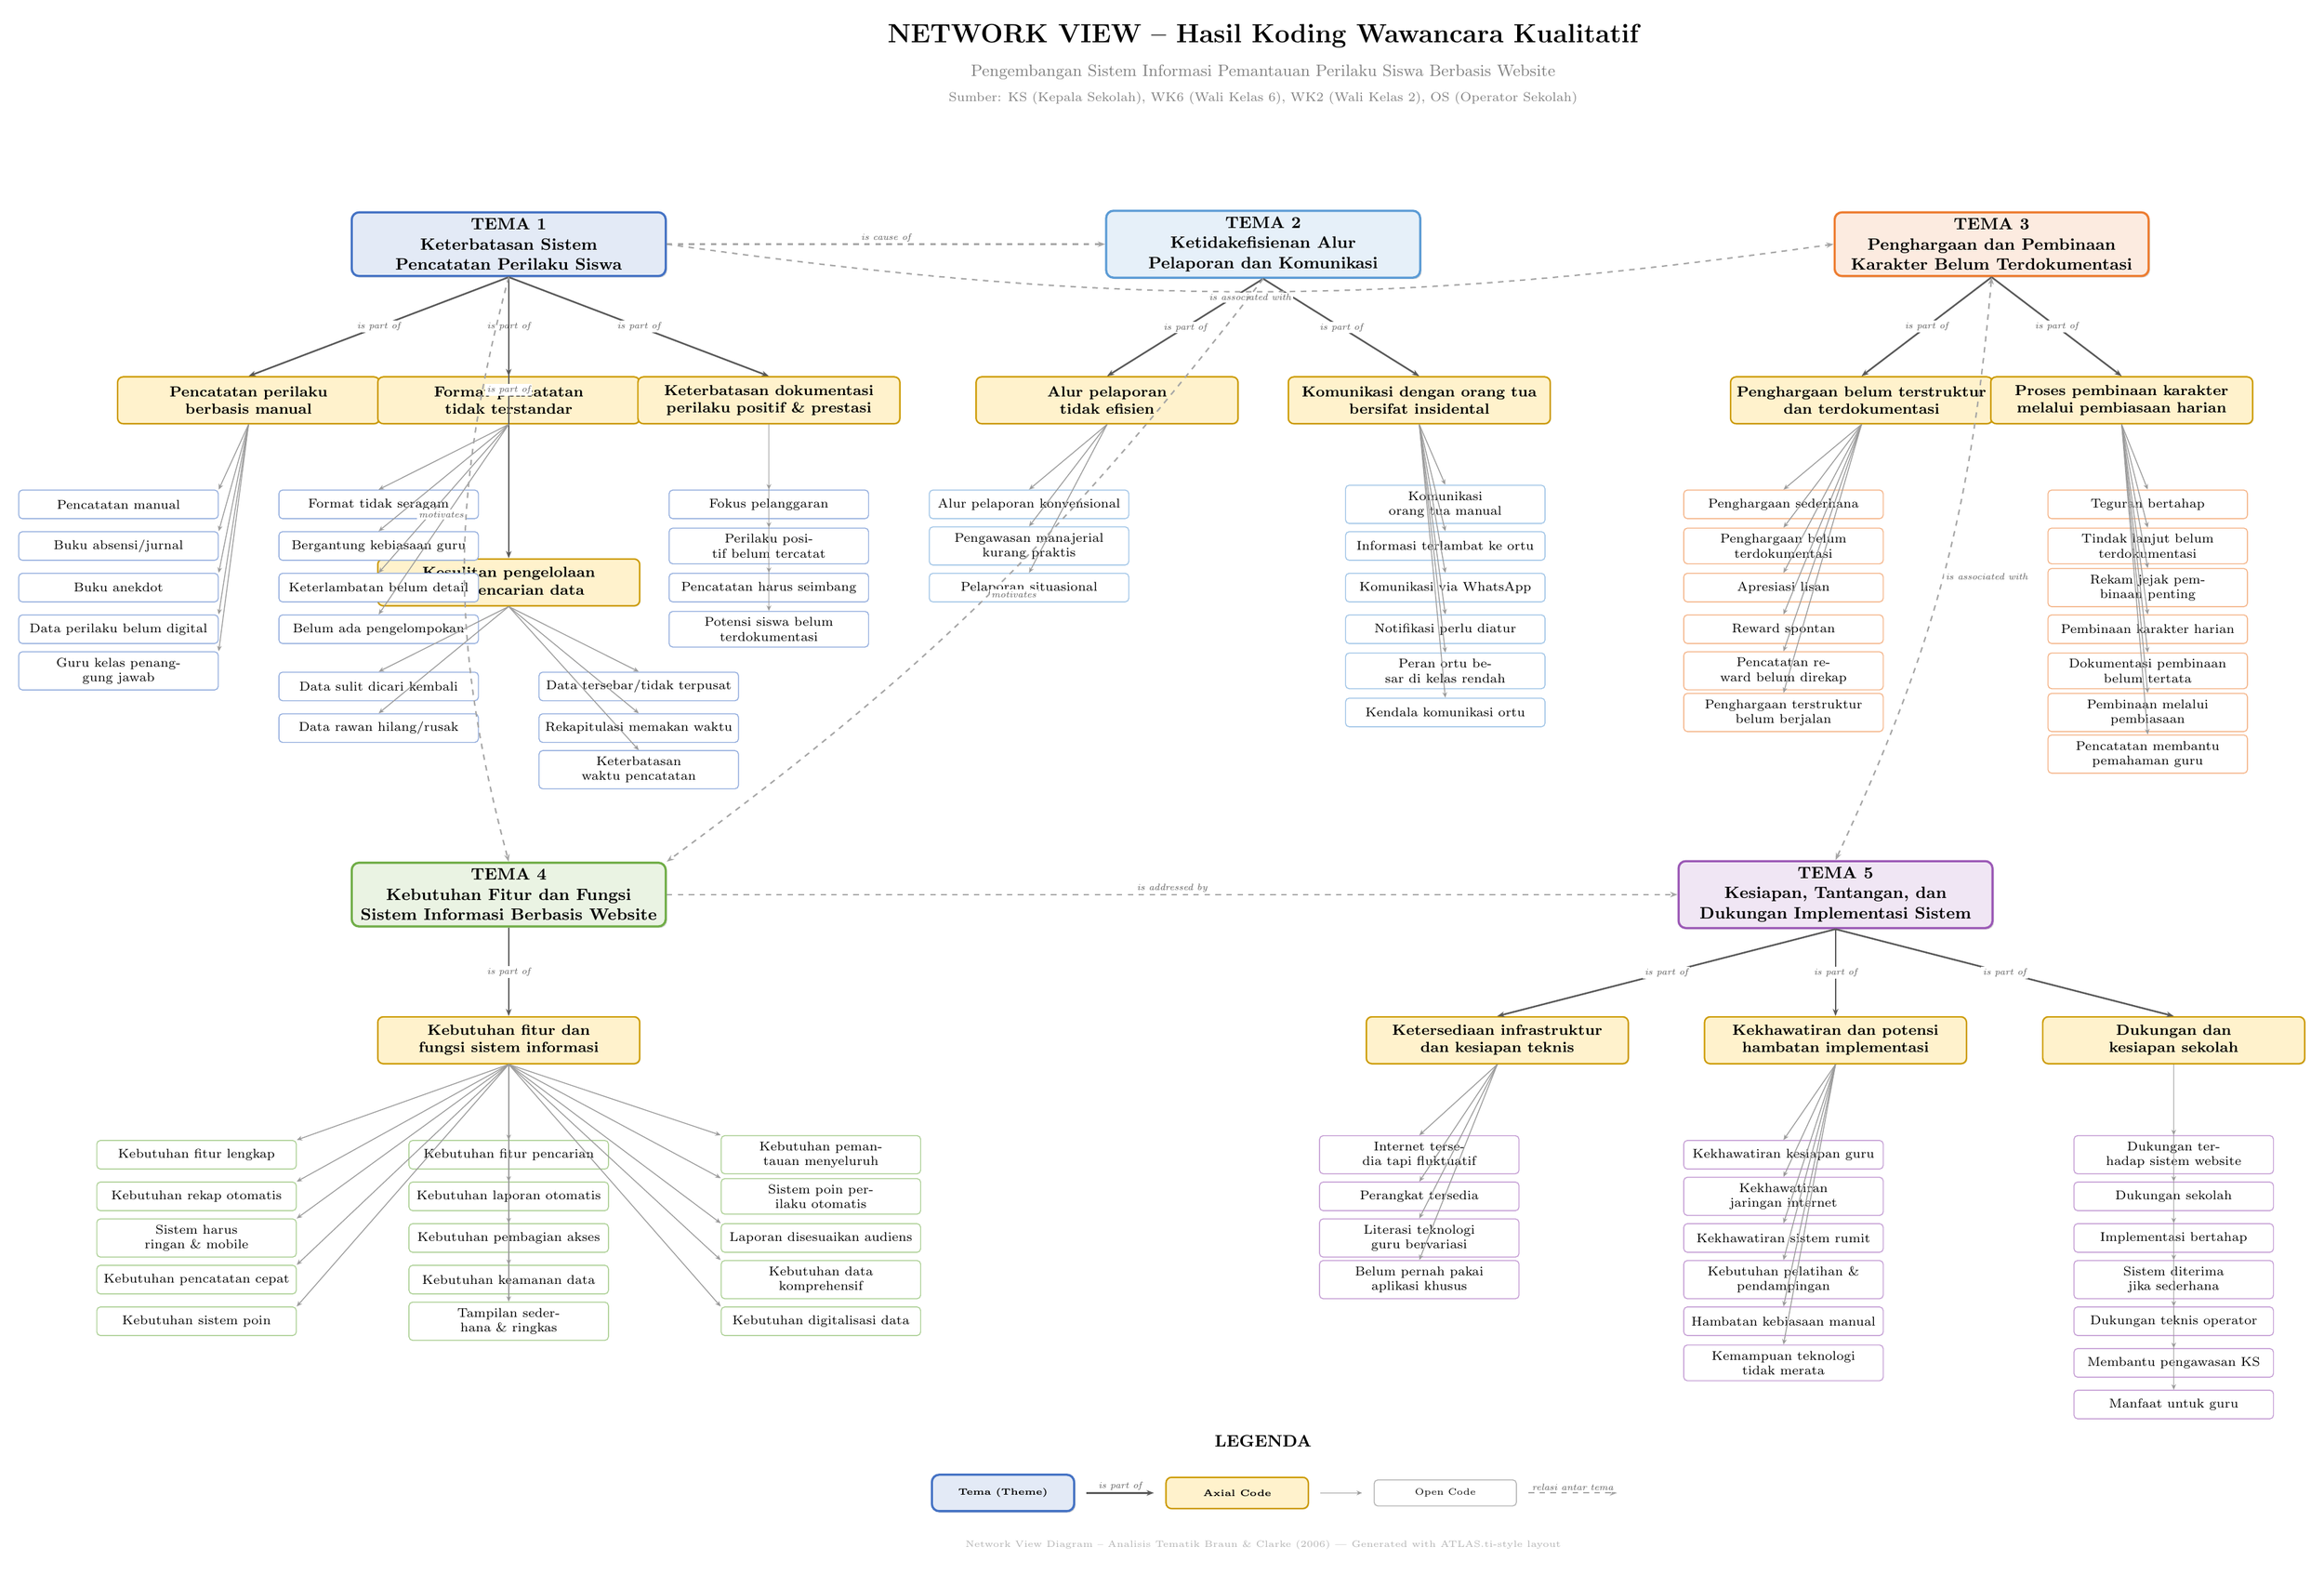
\begin{tikzpicture}[
    remember picture,
    % Node styles (ATLAS.ti inspired)
    theme/.style={
        rectangle, rounded corners=4pt,
        draw=#1, fill=#1!15, line width=1.2pt,
        text width=5.8cm, minimum height=1.2cm,
        align=center, font=\bfseries\small,
        drop shadow={shadow xshift=0.8pt, shadow yshift=-0.8pt, opacity=0.3}
    },
    axial/.style={
        rectangle, rounded corners=3pt,
        draw=axialcolor!80!black, fill=axialcolor!20, line width=0.8pt,
        text width=4.8cm, minimum height=0.9cm,
        align=center, font=\footnotesize\bfseries,
        drop shadow={shadow xshift=0.5pt, shadow yshift=-0.5pt, opacity=0.2}
    },
    opencode/.style={
        rectangle, rounded corners=2pt,
        draw=#1!60, fill=white, line width=0.5pt,
        text width=3.6cm, minimum height=0.55cm,
        align=center, font=\scriptsize
    },
    % Edge styles
    theme2axial/.style={
        -{Stealth[length=4pt, width=3pt]},
        line width=0.9pt, color=linkcolor,
    },
    axial2open/.style={
        -{Stealth[length=3pt, width=2.5pt]},
        line width=0.5pt, color=linkcolor!60,
    },
    relation/.style={
        font=\tiny\itshape, fill=white, inner sep=1pt, text=linkcolor
    },
]

% ===== TITLE =====
\node[font=\Large\bfseries, text=black] at (21, 18.5) {NETWORK VIEW -- Hasil Koding Wawancara Kualitatif};
\node[font=\small, text=gray] at (21, 17.8) {Pengembangan Sistem Informasi Pemantauan Perilaku Siswa Berbasis Website};
\node[font=\scriptsize, text=gray] at (21, 17.3) {Sumber: KS (Kepala Sekolah), WK6 (Wali Kelas 6), WK2 (Wali Kelas 2), OS (Operator Sekolah)};

% ===================================================================
% TEMA 1 (Top-Left) - Blue
% ===================================================================
\node[theme=theme1] (T1) at (6.5, 14.5)
    {TEMA 1\\Keterbatasan Sistem\\Pencatatan Perilaku Siswa};

% Axial codes for Tema 1
\node[axial] (A1) at (1.5, 11.5) {Pencatatan perilaku\\berbasis manual};
\node[axial] (A2) at (6.5, 11.5) {Format pencatatan\\tidak terstandar};
\node[axial] (A3) at (11.5, 11.5) {Keterbatasan dokumentasi\\perilaku positif \& prestasi};
\node[axial] (A4) at (6.5, 8.0) {Kesulitan pengelolaan\\dan pencarian data};

% Edges T1 -> Axials
\draw[theme2axial] (T1.south) -- node[relation, pos=0.5] {is part of} (A1.north);
\draw[theme2axial] (T1.south) -- node[relation, pos=0.5] {is part of} (A2.north);
\draw[theme2axial] (T1.south) -- node[relation, pos=0.5] {is part of} (A3.north);
\draw[theme2axial] (T1.south) -- node[relation, pos=0.4] {is part of} (A4.north);

% Open codes - A1
\node[opencode=theme1] (O1a) at (-1.0, 9.5) {Pencatatan manual};
\node[opencode=theme1] (O1b) at (-1.0, 8.7) {Buku absensi/jurnal};
\node[opencode=theme1] (O1c) at (-1.0, 7.9) {Buku anekdot};
\node[opencode=theme1] (O1d) at (-1.0, 7.1) {Data perilaku belum digital};
\node[opencode=theme1] (O1e) at (-1.0, 6.3) {Guru kelas penanggung jawab};

\draw[axial2open] (A1.south) -- (O1a.north east);
\draw[axial2open] (A1.south) -- (O1b.north east);
\draw[axial2open] (A1.south) -- (O1c.north east);
\draw[axial2open] (A1.south) -- (O1d.north east);
\draw[axial2open] (A1.south) -- (O1e.north east);

% Open codes - A2
\node[opencode=theme1] (O2a) at (4.0, 9.5) {Format tidak seragam};
\node[opencode=theme1] (O2b) at (4.0, 8.7) {Bergantung kebiasaan guru};
\node[opencode=theme1] (O2c) at (4.0, 7.9) {Keterlambatan belum detail};
\node[opencode=theme1] (O2d) at (4.0, 7.1) {Belum ada pengelompokan};

\draw[axial2open] (A2.south) -- (O2a.north);
\draw[axial2open] (A2.south) -- (O2b.north);
\draw[axial2open] (A2.south) -- (O2c.north);
\draw[axial2open] (A2.south) -- (O2d.north);

% Open codes - A3
\node[opencode=theme1] (O3a) at (11.5, 9.5) {Fokus pelanggaran};
\node[opencode=theme1] (O3b) at (11.5, 8.7) {Perilaku positif belum tercatat};
\node[opencode=theme1] (O3c) at (11.5, 7.9) {Pencatatan harus seimbang};
\node[opencode=theme1] (O3d) at (11.5, 7.1) {Potensi siswa belum terdokumentasi};

\draw[axial2open] (A3.south) -- (O3a.north);
\draw[axial2open] (A3.south) -- (O3b.north);
\draw[axial2open] (A3.south) -- (O3c.north);
\draw[axial2open] (A3.south) -- (O3d.north);

% Open codes - A4
\node[opencode=theme1] (O4a) at (4.0, 6.0) {Data sulit dicari kembali};
\node[opencode=theme1] (O4b) at (4.0, 5.2) {Data rawan hilang/rusak};
\node[opencode=theme1] (O4c) at (9.0, 6.0) {Data tersebar/tidak terpusat};
\node[opencode=theme1] (O4d) at (9.0, 5.2) {Rekapitulasi memakan waktu};
\node[opencode=theme1] (O4e) at (9.0, 4.4) {Keterbatasan waktu pencatatan};

\draw[axial2open] (A4.south) -- (O4a.north);
\draw[axial2open] (A4.south) -- (O4b.north);
\draw[axial2open] (A4.south) -- (O4c.north);
\draw[axial2open] (A4.south) -- (O4d.north);
\draw[axial2open] (A4.south) -- (O4e.north);

% ===================================================================
% TEMA 2 (Top-Right area) - Light Blue
% ===================================================================
\node[theme=theme2] (T2) at (21, 14.5)
    {TEMA 2\\Ketidakefisienan Alur\\Pelaporan dan Komunikasi};

% Axial codes for Tema 2
\node[axial] (A5) at (18.0, 11.5) {Alur pelaporan\\tidak efisien};
\node[axial] (A6) at (24.0, 11.5) {Komunikasi dengan orang tua\\bersifat insidental};

% Edges T2 -> Axials
\draw[theme2axial] (T2.south) -- node[relation, pos=0.5] {is part of} (A5.north);
\draw[theme2axial] (T2.south) -- node[relation, pos=0.5] {is part of} (A6.north);

% Open codes - A5
\node[opencode=theme2] (O5a) at (16.5, 9.5) {Alur pelaporan konvensional};
\node[opencode=theme2] (O5b) at (16.5, 8.7) {Pengawasan manajerial\\kurang praktis};
\node[opencode=theme2] (O5c) at (16.5, 7.9) {Pelaporan situasional};

\draw[axial2open] (A5.south) -- (O5a.north);
\draw[axial2open] (A5.south) -- (O5b.north);
\draw[axial2open] (A5.south) -- (O5c.north);

% Open codes - A6
\node[opencode=theme2] (O6a) at (24.5, 9.5) {Komunikasi orang tua manual};
\node[opencode=theme2] (O6b) at (24.5, 8.7) {Informasi terlambat ke ortu};
\node[opencode=theme2] (O6c) at (24.5, 7.9) {Komunikasi via WhatsApp};
\node[opencode=theme2] (O6d) at (24.5, 7.1) {Notifikasi perlu diatur};
\node[opencode=theme2] (O6e) at (24.5, 6.3) {Peran ortu besar di kelas rendah};
\node[opencode=theme2] (O6f) at (24.5, 5.5) {Kendala komunikasi ortu};

\draw[axial2open] (A6.south) -- (O6a.north);
\draw[axial2open] (A6.south) -- (O6b.north);
\draw[axial2open] (A6.south) -- (O6c.north);
\draw[axial2open] (A6.south) -- (O6d.north);
\draw[axial2open] (A6.south) -- (O6e.north);
\draw[axial2open] (A6.south) -- (O6f.north);

% ===================================================================
% TEMA 3 (Middle-Right) - Orange
% ===================================================================
\node[theme=theme3] (T3) at (35, 14.5)
    {TEMA 3\\Penghargaan dan Pembinaan\\Karakter Belum Terdokumentasi};

% Axial codes for Tema 3
\node[axial] (A7) at (32.5, 11.5) {Penghargaan belum terstruktur\\dan terdokumentasi};
\node[axial] (A8) at (37.5, 11.5) {Proses pembinaan karakter\\melalui pembiasaan harian};

% Edges T3 -> Axials
\draw[theme2axial] (T3.south) -- node[relation, pos=0.5] {is part of} (A7.north);
\draw[theme2axial] (T3.south) -- node[relation, pos=0.5] {is part of} (A8.north);

% Open codes - A7
\node[opencode=theme3] (O7a) at (31.0, 9.5) {Penghargaan sederhana};
\node[opencode=theme3] (O7b) at (31.0, 8.7) {Penghargaan belum terdokumentasi};
\node[opencode=theme3] (O7c) at (31.0, 7.9) {Apresiasi lisan};
\node[opencode=theme3] (O7d) at (31.0, 7.1) {Reward spontan};
\node[opencode=theme3] (O7e) at (31.0, 6.3) {Pencatatan reward belum direkap};
\node[opencode=theme3] (O7f) at (31.0, 5.5) {Penghargaan terstruktur\\belum berjalan};

\draw[axial2open] (A7.south) -- (O7a.north);
\draw[axial2open] (A7.south) -- (O7b.north);
\draw[axial2open] (A7.south) -- (O7c.north);
\draw[axial2open] (A7.south) -- (O7d.north);
\draw[axial2open] (A7.south) -- (O7e.north);
\draw[axial2open] (A7.south) -- (O7f.north);

% Open codes - A8
\node[opencode=theme3] (O8a) at (38.0, 9.5) {Teguran bertahap};
\node[opencode=theme3] (O8b) at (38.0, 8.7) {Tindak lanjut belum terdokumentasi};
\node[opencode=theme3] (O8c) at (38.0, 7.9) {Rekam jejak pembinaan penting};
\node[opencode=theme3] (O8d) at (38.0, 7.1) {Pembinaan karakter harian};
\node[opencode=theme3] (O8e) at (38.0, 6.3) {Dokumentasi pembinaan\\belum tertata};
\node[opencode=theme3] (O8f) at (38.0, 5.5) {Pembinaan melalui pembiasaan};
\node[opencode=theme3] (O8g) at (38.0, 4.7) {Pencatatan membantu\\pemahaman guru};

\draw[axial2open] (A8.south) -- (O8a.north);
\draw[axial2open] (A8.south) -- (O8b.north);
\draw[axial2open] (A8.south) -- (O8c.north);
\draw[axial2open] (A8.south) -- (O8d.north);
\draw[axial2open] (A8.south) -- (O8e.north);
\draw[axial2open] (A8.south) -- (O8f.north);
\draw[axial2open] (A8.south) -- (O8g.north);

% ===================================================================
% TEMA 4 (Bottom-Left) - Green
% ===================================================================
\node[theme=theme4] (T4) at (6.5, 2.0)
    {TEMA 4\\Kebutuhan Fitur dan Fungsi\\Sistem Informasi Berbasis Website};

% Axial codes for Tema 4
\node[axial] (A9) at (6.5, -0.8) {Kebutuhan fitur dan\\fungsi sistem informasi};

% Edges T4 -> Axials
\draw[theme2axial] (T4.south) -- node[relation, pos=0.5] {is part of} (A9.north);

% Open codes - A9 (spread in 3 columns)
\node[opencode=theme4] (O9a) at (0.5, -3.0) {Kebutuhan fitur lengkap};
\node[opencode=theme4] (O9b) at (0.5, -3.8) {Kebutuhan rekap otomatis};
\node[opencode=theme4] (O9c) at (0.5, -4.6) {Sistem harus ringan \& mobile};
\node[opencode=theme4] (O9d) at (0.5, -5.4) {Kebutuhan pencatatan cepat};
\node[opencode=theme4] (O9e) at (0.5, -6.2) {Kebutuhan sistem poin};

\node[opencode=theme4] (O9f) at (6.5, -3.0) {Kebutuhan fitur pencarian};
\node[opencode=theme4] (O9g) at (6.5, -3.8) {Kebutuhan laporan otomatis};
\node[opencode=theme4] (O9h) at (6.5, -4.6) {Kebutuhan pembagian akses};
\node[opencode=theme4] (O9i) at (6.5, -5.4) {Kebutuhan keamanan data};
\node[opencode=theme4] (O9j) at (6.5, -6.2) {Tampilan sederhana \& ringkas};

\node[opencode=theme4] (O9k) at (12.5, -3.0) {Kebutuhan pemantauan menyeluruh};
\node[opencode=theme4] (O9l) at (12.5, -3.8) {Sistem poin perilaku otomatis};
\node[opencode=theme4] (O9m) at (12.5, -4.6) {Laporan disesuaikan audiens};
\node[opencode=theme4] (O9n) at (12.5, -5.4) {Kebutuhan data komprehensif};
\node[opencode=theme4] (O9o) at (12.5, -6.2) {Kebutuhan digitalisasi data};

\draw[axial2open] (A9.south) -- (O9a.north east);
\draw[axial2open] (A9.south) -- (O9b.north east);
\draw[axial2open] (A9.south) -- (O9c.north east);
\draw[axial2open] (A9.south) -- (O9d.north east);
\draw[axial2open] (A9.south) -- (O9e.north east);
\draw[axial2open] (A9.south) -- (O9f.north);
\draw[axial2open] (A9.south) -- (O9g.north);
\draw[axial2open] (A9.south) -- (O9h.north);
\draw[axial2open] (A9.south) -- (O9i.north);
\draw[axial2open] (A9.south) -- (O9j.north);
\draw[axial2open] (A9.south) -- (O9k.north west);
\draw[axial2open] (A9.south) -- (O9l.north west);
\draw[axial2open] (A9.south) -- (O9m.north west);
\draw[axial2open] (A9.south) -- (O9n.north west);
\draw[axial2open] (A9.south) -- (O9o.north west);

% ===================================================================
% TEMA 5 (Bottom-Right) - Purple
% ===================================================================
\node[theme=theme5] (T5) at (32, 2.0)
    {TEMA 5\\Kesiapan, Tantangan, dan\\Dukungan Implementasi Sistem};

% Axial codes for Tema 5
\node[axial] (A10) at (25.5, -0.8) {Ketersediaan infrastruktur\\dan kesiapan teknis};
\node[axial] (A11) at (32, -0.8) {Kekhawatiran dan potensi\\hambatan implementasi};
\node[axial] (A12) at (38.5, -0.8) {Dukungan dan\\kesiapan sekolah};

% Edges T5 -> Axials
\draw[theme2axial] (T5.south) -- node[relation, pos=0.5] {is part of} (A10.north);
\draw[theme2axial] (T5.south) -- node[relation, pos=0.5] {is part of} (A11.north);
\draw[theme2axial] (T5.south) -- node[relation, pos=0.5] {is part of} (A12.north);

% Open codes - A10
\node[opencode=theme5] (O10a) at (24.0, -3.0) {Internet tersedia tapi fluktuatif};
\node[opencode=theme5] (O10b) at (24.0, -3.8) {Perangkat tersedia};
\node[opencode=theme5] (O10c) at (24.0, -4.6) {Literasi teknologi guru bervariasi};
\node[opencode=theme5] (O10d) at (24.0, -5.4) {Belum pernah pakai\\aplikasi khusus};

\draw[axial2open] (A10.south) -- (O10a.north);
\draw[axial2open] (A10.south) -- (O10b.north);
\draw[axial2open] (A10.south) -- (O10c.north);
\draw[axial2open] (A10.south) -- (O10d.north);

% Open codes - A11
\node[opencode=theme5] (O11a) at (31.0, -3.0) {Kekhawatiran kesiapan guru};
\node[opencode=theme5] (O11b) at (31.0, -3.8) {Kekhawatiran jaringan internet};
\node[opencode=theme5] (O11c) at (31.0, -4.6) {Kekhawatiran sistem rumit};
\node[opencode=theme5] (O11d) at (31.0, -5.4) {Kebutuhan pelatihan \&\\pendampingan};
\node[opencode=theme5] (O11e) at (31.0, -6.2) {Hambatan kebiasaan manual};
\node[opencode=theme5] (O11f) at (31.0, -7.0) {Kemampuan teknologi\\tidak merata};

\draw[axial2open] (A11.south) -- (O11a.north);
\draw[axial2open] (A11.south) -- (O11b.north);
\draw[axial2open] (A11.south) -- (O11c.north);
\draw[axial2open] (A11.south) -- (O11d.north);
\draw[axial2open] (A11.south) -- (O11e.north);
\draw[axial2open] (A11.south) -- (O11f.north);

% Open codes - A12
\node[opencode=theme5] (O12a) at (38.5, -3.0) {Dukungan terhadap sistem website};
\node[opencode=theme5] (O12b) at (38.5, -3.8) {Dukungan sekolah};
\node[opencode=theme5] (O12c) at (38.5, -4.6) {Implementasi bertahap};
\node[opencode=theme5] (O12d) at (38.5, -5.4) {Sistem diterima jika sederhana};
\node[opencode=theme5] (O12e) at (38.5, -6.2) {Dukungan teknis operator};
\node[opencode=theme5] (O12f) at (38.5, -7.0) {Membantu pengawasan KS};
\node[opencode=theme5] (O12g) at (38.5, -7.8) {Manfaat untuk guru};

\draw[axial2open] (A12.south) -- (O12a.north);
\draw[axial2open] (A12.south) -- (O12b.north);
\draw[axial2open] (A12.south) -- (O12c.north);
\draw[axial2open] (A12.south) -- (O12d.north);
\draw[axial2open] (A12.south) -- (O12e.north);
\draw[axial2open] (A12.south) -- (O12f.north);
\draw[axial2open] (A12.south) -- (O12g.north);

% ===================================================================
% INTER-THEME RELATIONSHIPS (dashed, ATLAS.ti style)
% ===================================================================
\draw[dashed, thick, color=gray!70, -{Stealth[length=4pt]}]
    (T1.east) -- node[relation, pos=0.5, above, fill=white] {is cause of} (T2.west);

\draw[dashed, thick, color=gray!70, -{Stealth[length=4pt]}]
    (T1.east) to[bend right=8] node[relation, pos=0.5, below, fill=white] {is associated with} (T3.west);

\draw[dashed, thick, color=gray!70, -{Stealth[length=4pt]}]
    (T1.south) to[bend right=15] node[relation, pos=0.4, left, fill=white] {motivates} (T4.north);

\draw[dashed, thick, color=gray!70, -{Stealth[length=4pt]}]
    (T2.south) to[bend left=8] node[relation, pos=0.5, right, fill=white] {motivates} (T4.north east);

\draw[dashed, thick, color=gray!70, -{Stealth[length=4pt]}]
    (T4.east) -- node[relation, pos=0.5, above, fill=white] {is addressed by} (T5.west);

\draw[dashed, thick, color=gray!70, {Stealth[length=4pt]}-{Stealth[length=4pt]}]
    (T3.south) to[bend left=10] node[relation, pos=0.5, right, fill=white] {is associated with} (T5.north);

% ===================================================================
% LEGEND
% ===================================================================
\node[font=\small\bfseries] at (21, -8.5) {LEGENDA};

\node[theme=theme1, text width=2.5cm, minimum height=0.7cm, font=\tiny\bfseries] (leg1) at (16, -9.5) {Tema (Theme)};
\node[axial, text width=2.5cm, minimum height=0.6cm, font=\tiny\bfseries] (leg2) at (20.5, -9.5) {Axial Code};
\node[opencode=gray, text width=2.5cm, minimum height=0.5cm, font=\tiny] (leg3) at (24.5, -9.5) {Open Code};

\draw[theme2axial] (17.6, -9.5) -- (18.9, -9.5) node[relation, pos=0.5, above] {is part of};
\draw[axial2open] (22.1, -9.5) -- (22.9, -9.5);
\draw[dashed, thick, color=gray!70, -{Stealth[length=4pt]}] (26.1, -9.5) -- (27.8, -9.5) node[relation, pos=0.5, above] {relasi antar tema};

% Source info
\node[font=\tiny, text=gray!60] at (21, -10.5) {Network View Diagram -- Analisis Tematik Braun \& Clarke (2006) | Generated with ATLAS.ti-style layout};

\end{tikzpicture}

\end{document}
